% anumana — honest-benchmark workshop paper.
%
% Self-contained: compiles with a standard TeX install (Overleaf, MacTeX,
% TeX Live) via `pdflatex main.tex` -- no bibtex pass needed (manual
% thebibliography). Conservative preamble on purpose.
%
% For camera-ready submission to NeurIPS ICBINB (the target venue), see
% paper/README.md: drop in the official `neurips_<year>.sty` (ICBINB uses
% the NeurIPS style), switch \documentclass, and the body below is
% unchanged.
\documentclass[11pt]{article}

\usepackage[utf8]{inputenc}
\usepackage[T1]{fontenc}
\usepackage[margin=1in]{geometry}
\usepackage{amsmath}
\usepackage{booktabs}
\usepackage{graphicx}
\usepackage{xcolor}
\usepackage[colorlinks=true,allcolors=blue]{hyperref}

\title{Contextual Optimization for Scene-Adaptive Multi-Target\\
Tracker Tuning: An Honest Benchmark}
\author{Harsh Dhingra\\
\texttt{dhingrah02@gmail.com}\\
\small\url{https://github.com/Harsh-Dhingra/anumana}}
\date{2026}

\begin{document}
\maketitle

\begin{abstract}
Multi-target tracking pipelines expose tunable parameters (association
gate size, process-noise scaling, hypothesis-pruning thresholds) whose
optimal values depend on the scene. Prior work
\citep{stephan2022,ott2022} tunes these online with reinforcement and
meta-RL. We ask a narrower, practical question: \emph{does conditioning
on cheap scene-context features actually beat simply re-tuning per
scenario?} We build the first open, reproducible benchmark for
scene-adaptive tracker autotuning---a JPDA tracker on Stone Soup over a
parameterised counter-UAS swarm grid---and compare random search,
per-scenario Bayesian optimization, one-shot contextual BO, a warm-start
hybrid, and a PPO policy, with bootstrap confidence intervals on
held-out scenes ($n{=}12$). \textbf{Our headline result is negative and
specific}: one-shot \emph{contextual} BO is the \emph{worst} learned
method on average (mean $75.0$ vs.\ random search $70.1$) and is unsafe
under clutter distribution shift---on an out-of-distribution cell its
unbounded GP posterior mean yields sub-default proposals. Cheap
per-scenario BO ($61.5$), a warm-start hybrid ($59.9$), and a PPO policy
($61.8$) are statistically indistinguishable; all tuning beats untuned
defaults ($90.9$) by ${\approx}32\text{--}34\%$. We additionally note,
as a conjecture from limited data, that a context-conditioned RL policy
degrades more gracefully than the GP. We release the benchmark and code,
and are explicit throughout about which claims are significant, which
are nulls, and which are conjectures.
\end{abstract}

\section{Introduction}

Classical multi-target trackers---JPDA, MHT, IMM-Kalman---carry
hand-tuned parameters set once by engineers and held fixed regardless of
the scene. In counter-UAS settings (dense small-UAS swarms, low SNR,
high clutter, correlated motion) a single configuration is provably
suboptimal: the regime that fits three aircraft at \SI{}{30~km} does not
fit a hundred drones at \SI{}{3~km}.

Two recent works tune these parameters adaptively with deep RL
\citep{stephan2022} and uncertainty-aware meta-RL with a scene
``context prior'' \citep{ott2022}. Both report large gains over fixed
parameters; both require ${\sim}10^6$ training rollouts and neither
released code.

A natural hypothesis follows: a \emph{sample-efficient} contextual
Bayesian optimizer should match RL-based scene-adaptive tuning at a tiny
fraction of the training cost. We set out to demonstrate exactly that.
\textbf{We could not.} This paper reports what we found instead, and
contributes the open testbed that let us find it:

\begin{itemize}
\item \textbf{A reproducible benchmark} for scene-adaptive MTT tracker
autotuning: a seeded counter-UAS swarm scenario generator, a JPDA
tracker on the open-source Stone Soup framework, five tuning strategies,
and a metrics + bootstrap-CI evaluation harness
(Sections~\ref{sec:setup}--\ref{sec:protocol}).
\item \textbf{A negative empirical finding}, stated honestly with
statistics: one-shot contextual BO is the \emph{worst} learned method
(below per-scenario random search) and is unsafe under clutter shift; a
warm-start hybrid accelerates early BO but does not improve the
converged answer; cheap per-scenario BO, warm-start, and PPO are
mutually indistinguishable. Each finding is tagged by evidential status
(Sections~\ref{sec:results}--\ref{sec:discussion}).
\item \textbf{Open code and archived results} so the comparison is
extensible---the artifact prior work omitted
(Section~\ref{sec:artifact}).
\end{itemize}

\section{Related work}

\textbf{Scene-adaptive tracker tuning.} \citet{stephan2022} tune
Unscented-Kalman tracking parameters with deep RL and scene-dependent
reward formulations. \citet{ott2022} extend this with uncertainty-based
meta-RL and a 2-D ``context prior'' (mean/std of the range--angle
image) for cross-room generalization plus out-of-distribution
detection; ${\sim}4{\times}10^6$ training steps; no public code. Our
context features (target density, measurement rate, dispersion) are the
same idea in a different modality, and our contextual GP plays the role
of their context-conditioned policy. We differ in method (Bayesian
optimization vs.\ meta-RL), tracker (JPDA on Stone Soup vs.\ UKF on a
proprietary FMCW pipeline), and reproducibility (open).

\textbf{BO for tracker hyperparameters.} \citet{fleck2021} tune a GM-PHD
tracker offline with TPE/SMAC/Spearmint---per-scenario, no context, no
transfer. We include this regime as our \texttt{vanilla\_bo} baseline.

\textbf{Contextual Bayesian optimization.} \citet{krause2011} introduced
contextual GP-UCB; transfer/meta-BO surveys \citep{bai2023} situate
context-conditioned BO among warm-starting and multi-task methods. We
apply the standard contextual-GP machinery; the contribution is the
honest empirical test on a tracking problem, not new BO methodology.

\section{Problem setup}
\label{sec:setup}

\textbf{Tracker.} JPDA (\texttt{stonesoup} 1.8): Kalman
predictor/updater, \texttt{PDAHypothesiser}, \texttt{JPDA} data
associator, \texttt{GNNWith2DAssignment} +
\texttt{MultiMeasurementInitiator}, \texttt{CovarianceBasedDeleter}.
Tunable parameters: ellipsoidal gate size, process-noise scaling,
hypothesis pruning threshold (3-D unit-cube search space).

\textbf{Scenarios.} \texttt{SwarmScenario}: $N$ targets enter one edge
of a square arena flying roughly across it, Gaussian process noise as a
maneuver proxy, uniform clutter, configurable detection probability.
Materialised once and replayed deterministically (numpy global RNG
snapshot/restore), so every method sees an identical scene and runs are
reproducible.

\textbf{Grid.} A \emph{train} set of 6 cells and a \emph{held-out} set
of 4 cells over (num\_targets $\times$ clutter\_rate $\times$
maneuver\_intensity). Held-out includes two interior-interpolation cells
and two extrapolation cells (clutter and maneuver beyond the training
support) to probe distribution shift.

\textbf{Metric.} Composite reward $=$ mean OSPA $+\,5\cdot(\text{ID
switches}) + 5\cdot(\text{fragmentations})$, lower is better.
OSPA/GOSPA via Stone Soup's metric generators; ID switches and
fragmentation via greedy per-timestep nearest-neighbour assignment.

\section{Methods compared}

\begin{enumerate}
\item \textbf{default} --- Stone Soup JPDA default parameters, no tuning.
\item \textbf{RandomSearch} --- $K$ per-scenario uniform draws, best.
\item \textbf{BayesOpt} --- $K$ per-scenario GP-UCB trials (BoTorch
\texttt{SingleTaskGP}), best.
\item \textbf{ContextualBayesOpt} --- GP over the joint (params,
context) space fit on a transfer pool from the train grid; one-shot
posterior-mean proposal for a held-out scene (no per-scenario trials).
\item \textbf{WarmStartBayesOpt} --- per-scenario GP-UCB whose trial-0
is the contextual proposal and whose random bootstrap is shortened.
\item \textbf{PPO} --- single-step contextual-bandit policy
(Stable-Baselines3, VecNormalize over context), trained on the train
grid; one-shot deterministic proposal.
\end{enumerate}

\section{Experimental protocol}
\label{sec:protocol}

Train pool: 6 cells $\times$ 3 seeds $\times$ 8 BO trials. PPO:
$2{\times}10^4$ environment steps. Held-out evaluation: 4 cells $\times$
3 seeds ($n{=}12$ points). $K{=}8$ trials for per-scenario methods.
Each held-out scene is evaluated by all six methods on the \emph{same}
seeded scenario. We report mean composite with percentile bootstrap
95\% CIs (5000 resamples). Scenarios are fully seeded; parallel and
serial execution are bit-identical.

\section{Results}
\label{sec:results}

\begin{table}[h]
\centering
\caption{Benchmark ($n{=}12$ held-out points; mean composite, lower is
better; percentile bootstrap 95\% CI, 5000 resamples).}
\begin{tabular}{lccc}
\toprule
Method & mean & 95\% CI & std \\
\midrule
Default params & 90.87 & [80.81, 102.13] & 18.60 \\
Random search ($K{=}8$) & 70.12 & [58.47, 79.66] & 18.66 \\
Vanilla BO ($K{=}8$) & 61.53 & [49.32, 71.84] & 20.31 \\
\textbf{Contextual BO (one-shot)} & \textbf{75.01} &
\textbf{[58.30, 94.93]} & \textbf{32.25} \\
Warm-start BO ($K{=}8$) & 59.85 & [48.10, 70.26] & 19.63 \\
PPO (one-shot) & 61.76 & [49.18, 72.83] & 20.75 \\
\bottomrule
\end{tabular}
\label{tab:main}
\end{table}

\begin{figure}[h]
\centering
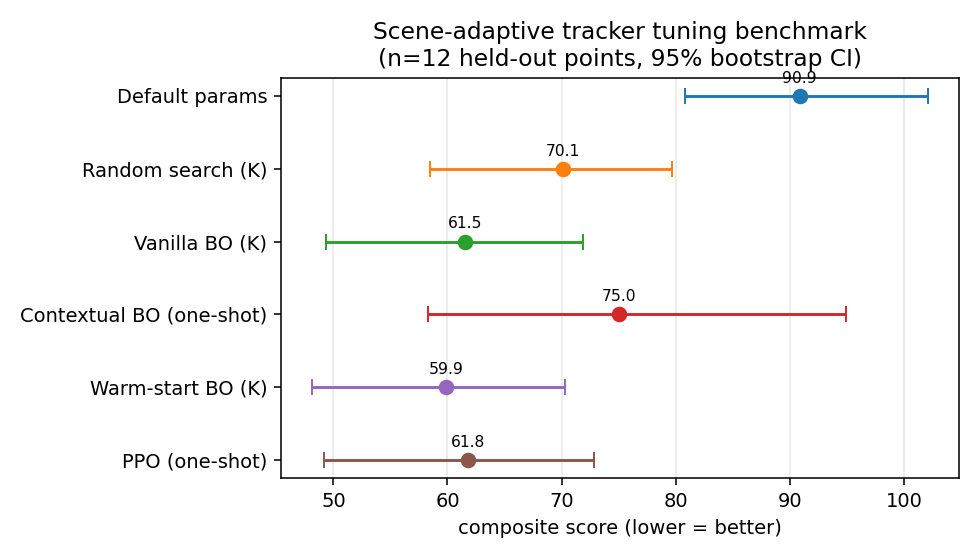
\includegraphics[width=0.7\linewidth]{figs/benchmark_forest.png}
\caption{Method means with bootstrap 95\% CIs.}
\label{fig:forest}
\end{figure}

\begin{figure}[h]
\centering
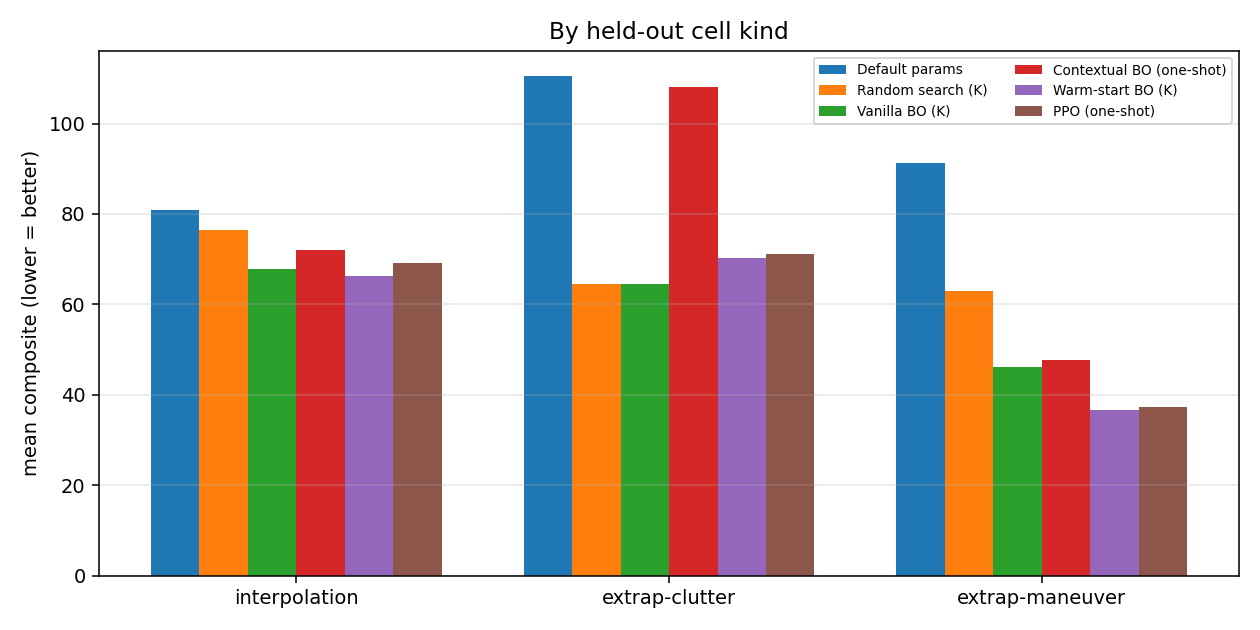
\includegraphics[width=0.95\linewidth]{figs/benchmark_by_kind.png}
\caption{Per-cell-kind breakdown (interpolation vs.\ extrap-clutter
vs.\ extrap-maneuver). Contextual BO's blow-up is the extrap-clutter
group.}
\label{fig:bykind}
\end{figure}

\textbf{F1 --- tuning beats no tuning (significant).} Default's CI lower
bound (80.81) sits above every tuned method's CI upper bound;
${\approx}32\text{--}34\%$ improvement.

\textbf{F2 --- one-shot contextual BO is the worst learned method on
average and fails catastrophically under clutter shift (headline).} Its
mean (75.0) is worst among learned methods---worse than random
search---and it carries ${\sim}1.6\times$ the variance of every other
method; this ranking is robust across all $n{=}12$ points. The dramatic
``worse than untuned default'' behaviour is precisely scoped: it occurs
on the single clutter-extrapolation cell ($N{=}10$, clutter${=}8$,
training clutter capped at 6), on 2 of its 3 seeds (154.7 and 109.7
vs.\ default 135.8 and 108.4; the third seed, 60.0, is fine). A poor
interpolation point (98.7) also contributes. The mechanism is the
unbounded GP posterior mean confidently extrapolating outside training
support. We do not claim contextual BO \emph{always} underperforms
defaults---we claim it is the worst learned method in aggregate and is
\emph{unsafe} (high-variance, capable of sub-default proposals)
precisely where an autotuner most needs to be safe.

\textbf{F3 --- among per-scenario / hybrid methods, nothing beats
anything (null).} Vanilla BO (61.5), warm-start (59.9), PPO one-shot
(61.8) are statistically indistinguishable (heavily overlapping CIs);
warm-start's best mean is within noise (consistent with a pre-registered
warm-start gate that failed its ${\le}4$-trial criterion). This is a
null result, reported as one.

\textbf{F4 --- a conjecture: context-conditioned RL appears to degrade
more gracefully than the context-conditioned GP.} On the same
clutter-extrapolation cell, PPO returns 60.4 / 90.2 / 62.9 versus
contextual BO's 154.7 / 109.7 / 60.0---PPO degrades but does not
collapse. This is \textbf{3 points per method on one cell}; we present
it as a hypothesis, not a result. A plausible mechanism is that PPO's
bounded (tanh-squashed) action head and clipped, normalised
observations cap how bad a proposal can be, whereas an unconstrained GP
posterior mean has no such floor. Confirming this would need a dedicated
experiment (more extrapolation cells, ablating the action bound).

\textbf{Statistical honesty.} We state the evidential status of each
finding explicitly, because this paper criticizes prior work for
overclaiming and must not repeat it. \textbf{F1} is statistically
supported (non-overlapping CIs). \textbf{F2} is a ranking + variance
finding; the ``sub-default'' instances are 2 of 3 seeds on one cell and
are reported as such, not generalised. \textbf{F3} is a null---we do
not claim any method is best. \textbf{F4} is an explicitly labelled
conjecture from 3 points per method on a single cell. $n{=}12$ is
sufficient for F1 (significant), F2 (a variance/ranking story more seeds
only sharpen), and F3 (a null more seeds only reconfirm); it is
\emph{not} sufficient to elevate F4 beyond a conjecture, and we do not.

\section{Discussion}
\label{sec:discussion}

\textbf{One-shot contextual BO is not merely ``not better''---it is the
worst learned method and is dangerous under distribution shift.} The
original hypothesis was that a sample-efficient contextual GP would
match RL-based scene-adaptive tuning. It does not. Worse, its failure
mode is unsafe: the GP posterior mean is overconfident outside its
training support, so on out-of-distribution clutter it proposes
parameters worse than doing no tuning at all. For an operational
autotuner this is the opposite of a safe default.

\textbf{RL \emph{may} extrapolate more gracefully than the GP
(conjecture).} On the one clutter-extrapolation cell PPO degrades but
does not collapse while contextual BO does (F4). We \emph{conjecture}
this is because PPO's bounded action head and clipped observations cap
how bad a proposal can be, whereas an unconstrained GP posterior mean
has no floor. We deliberately do not present this as a result---it
rests on 3 points per method on one cell. If it holds under a dedicated
experiment it has a clean operational implication: when one-shot context
conditioning is unavoidable, prefer a bounded learned policy to a GP
posterior mean. Either way, neither one-shot method beats cheap
per-scenario BO.

\textbf{Warm-starting accelerates but does not improve.} Seeding
per-scenario BO from the contextual prior reaches a given quality in
fewer trials, but the converged solution is unchanged (warm-start
$59.9\approx$ vanilla $61.5$, CIs overlapping) and the prior hurts under
the same clutter shift.

\textbf{Tuning matters; the choice among reasonable per-scenario methods
does not.} Any tuning beats default by ${\approx}32\text{--}34\%$
(significant). Among vanilla BO, warm-start, and PPO the differences are
within noise at $n{=}12$. The honest operational takeaway: spend the
engineering on \emph{some} per-scenario tuning loop, not on
context-conditioned one-shot prediction.

\textbf{Why report this.} The field has two papers claiming large gains
from scene-adaptive RL tuning and no open baseline. A reproducible
benchmark showing that the cheap baseline is hard to beat is a useful
corrective and a foundation others can build on.

\section{The artifact}
\label{sec:artifact}

\texttt{anumana} (BSD-3-Clause,
\url{https://github.com/Harsh-Dhingra/anumana}): seeded counter-UAS
swarm scenario generator, instrumented JPDA tracker, metrics pipeline,
five tuning optimizers behind one \texttt{AutoTuner} loop, a
joblib-parallel grid harness, and the benchmark + plotting scripts. All
experiment results are archived under \texttt{results/} with
per-experiment READMEs and reproduce commands. CI runs the test suite
on Python 3.11/3.12.

\section{Limitations and future work}

\begin{itemize}
\item Synthetic Stone Soup scenarios only; no real radar data.
\item Single tracker family (JPDA); MHT/IMM/RFS untested.
\item 3-D parameter space; IMM model weights and track init/delete
thresholds excluded.
\item $n{=}12$ held-out points (4 cells $\times$ 3 seeds). Adequate for
F1 (significant) and F2 (a ranking/variance story); insufficient to
elevate F4 past a conjecture. Expandable to 5+ seeds cheaply (PPO is
cached).
\item Hand-engineered context features; learned/embedding contexts and
an OOD-aware fallback (à la \citet{ott2022}'s uncertainty gating) are
open directions that could plausibly rescue the one-shot regime---an
OOD detector that declined to act on the clutter-extrapolation cell
would remove F2's catastrophic instances.
\item ${\approx}10\text{--}15\%$ residual prior-art risk: SPIE Defense,
IEEE Radar Conf, and non-English radar venues not exhaustively combed.
\end{itemize}

\begin{thebibliography}{9}

\bibitem[Bai et al.(2023)]{bai2023}
T.~Bai et al.
\newblock Transfer Learning for Bayesian Optimization: A Survey.
\newblock \emph{arXiv:2302.05927}, 2023.

\bibitem[Balandat et al.(2020)]{balandat2020}
M.~Balandat et al.
\newblock BoTorch: A Framework for Efficient Monte-Carlo Bayesian
Optimization.
\newblock \emph{NeurIPS}, 2020.

\bibitem[Fleck \& Zoellner(2021)]{fleck2021}
T.~Fleck and J.~M. Zoellner.
\newblock Tuning Multi Object Tracking Systems using Bayesian
Optimization.
\newblock \emph{24th Int. Conf. on Information Fusion (FUSION)}, 2021.

\bibitem[Krause \& Ong(2011)]{krause2011}
A.~Krause and C.~S. Ong.
\newblock Contextual Gaussian Process Bandit Optimization.
\newblock \emph{NeurIPS}, 2011.

\bibitem[Ott et al.(2022)]{ott2022}
J.~Ott, L.~Servadei, G.~Mauro, T.~Stadelmayer, A.~Santra, R.~Wille.
\newblock Uncertainty-based Meta-Reinforcement Learning for Robust
Radar Tracking.
\newblock \emph{arXiv:2210.14532}, 2022.

\bibitem[Schulman et al.(2017)]{schulman2017}
J.~Schulman, F.~Wolski, P.~Dhariwal, A.~Radford, O.~Klimov.
\newblock Proximal Policy Optimization Algorithms.
\newblock \emph{arXiv:1707.06347}, 2017.

\bibitem[Stephan et al.(2022)]{stephan2022}
M.~Stephan, L.~Servadei, J.~Arjona-Medina, A.~Santra, R.~Wille,
G.~Fischer.
\newblock Scene-adaptive radar tracking with deep reinforcement
learning.
\newblock \emph{Machine Learning with Applications}, 8:100284, 2022.

\end{thebibliography}

\end{document}
